\subsection{\texorpdfstring{W+jets Background Estimation in $\tauTau$ Channel}{W+jets Background Estimation in tau-tau Channel}}
\subsubsection{Method Description}
As shown in table~\ref{tbl:cutflowtable}, the number of W+jets events surviving 
the selection cuts are found to be zero in search \binone or 0.43$\pm$0.40 in search \bintwo. 
Therefore, the statistical uncertainties on the expected yields of W+jets events
are huge, e.g. it reaches to 93\% in \bintwo. 
 The statistical uncertainty on the yields for W+jets events can be improved by extracting 
the $\mttwo$ or $\SumMT$ cut efficiency, depending on the search bins, in a sample with more 
statistics. To make this sample, some cuts with small effects on the search variables are 
relaxed. Various samples with different relaxed cuts are examined to check the idea of small correlation 
between search variable and relaxed cuts. In the next section, the validation of this method will be discussed.\\
When the cut efficiency for the $\mttwo$ or $\SumMT$ variable is found, then it is multiplied by the W+jets 
yields before cutting on the search variable. This means, according to table~\ref{tbl:cutflowtable}, the cut efficiency for 
$\mttwo$ ($\SumMT$) found in a relaxed sample should be multiplied by 31.93 (29.13) to get an 
estimate for the W+jets events in search \binone (search \bintwo).\\
The systematics that can be assigned to this method is the maximum
variation of the estimations among those relaxed samples.
\subsubsection{Method Validation}
The idea is to check the effect of three (four) set of cuts independently, 
on the \mttwo or \SumMT cut efficiency in search \binone (\bintwo). 
Therefore, starting with a baseline selection cuts, defined as two 
medium-isolated opposite sign \Tau's, the $\mttwo$ or $\SumMT$ cut 
efficiency is calculated, for those events passing and failing the following list of cuts (one-by-one)
\begin{itemize}
\item lepton veto
\item $\mindphifour>$ 1
\item Z veto 
\item b-jet veto (only for search \bintwo)
\end{itemize}

 The cut efficiencies and final estimated values for 
search \binone can be found in figure~\ref{fig:wjets_1}. 
\begin{figure}[iHhtb]
\centering
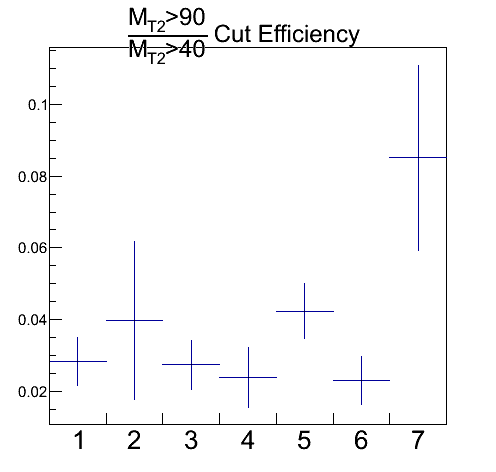
\includegraphics[angle=0,scale=0.35]{TauTauFigs/eff_bin1.png}
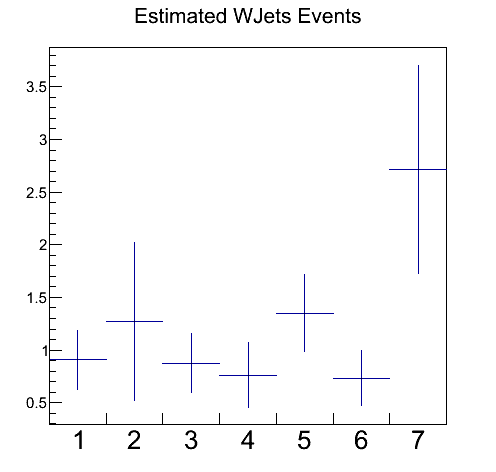
\includegraphics[angle=0,scale=0.35]{TauTauFigs/est_bin1.png} \\
\caption{The distribution of $\frac{\mttwo>90}{\mttwo>40}$ cut 
efficiency (left) and final estimated W+jets events (right) in search \binone.
 The first bin corresponds to the sample of events passing the baseline selection cuts. 
The next six bins correspond to the samples where passing and failing the 
list of cuts mentioned in the text, respectively.}
\label{fig:wjets_1}
\end{figure}

The same plots for search \bintwo are shown in figure~\ref{fig:wjets_2}. These plots can be used to verify the method. 
\begin{figure}[iHhtb]
\centering
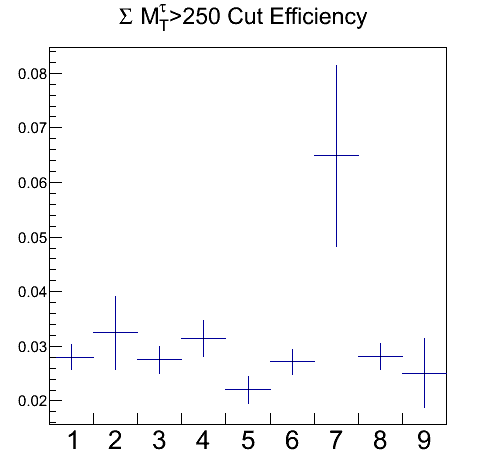
\includegraphics[angle=0,scale=0.35]{TauTauFigs/eff_bin2.png}
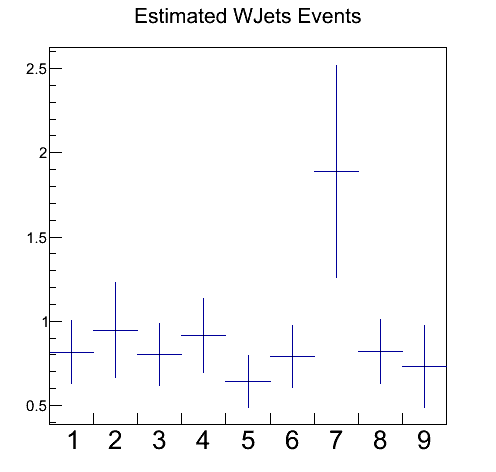
\includegraphics[angle=0,scale=0.35]{TauTauFigs/est_bin2.png} \\
\caption{The distribution of $\SumMT>250$ cut 
efficiency (left) and final estimated W+jets events (right) in search \bintwo.
 The first bin corresponds to the sample of events passing the baseline selection cuts. 
The next eight bins correspond to the samples where passing and failing the 
list of cuts mentioned in the text, respectively.}
\label{fig:wjets_2}
\end{figure}

[{\bf FIXME} update the extracted values from the plots, according to the discussion in the SUSY meeting] A summary of the estimated W+jets events can be found in table~\ref{tbl:wjetsEstimation}. 

\begin{table}
\begin{center}
\begin{tabular}{lc}
\hline\hline
& W+jets Estimated Results\\
\hline
\binone & 0.66 $\pm$ 0.15 (stat.) $\pm$ 0.20 (sys.)\\
\hline
\bintwo & 0.80 $\pm$ 0.20 (stat.) $\pm$ 0.10 (sys.)\\
\hline\hline 
\end{tabular}
\caption{The W+jets estimation results. The systematics assigned to each search bin 
comes from the maximum variation of the estimations on that bin (neglecting the 7th bin) [{\bf FIXME} justify this with a plot: comment from SUSY meeting].}
\label{tbl:wjetsEstimation}
\end{center}
\end{table}

\subsubsection{MC Validation for W+jets}
To verify that the MC has a good description of the W+jets events and it can be trusted for both shape and normalization, a data/MC comparison 
is done in a W+jets enriched sample. To enrich the sample, \muTau selection is done with the following modifications:
\begin{itemize}
\item $\mu$ and \Tau are same sign.
\item B-tagged jets with CSVL are vetoed.
\item \Tau isolation changed from Tight to Loose.
\end{itemize}
Figure 
\begin{figure}[htbp]
\centering
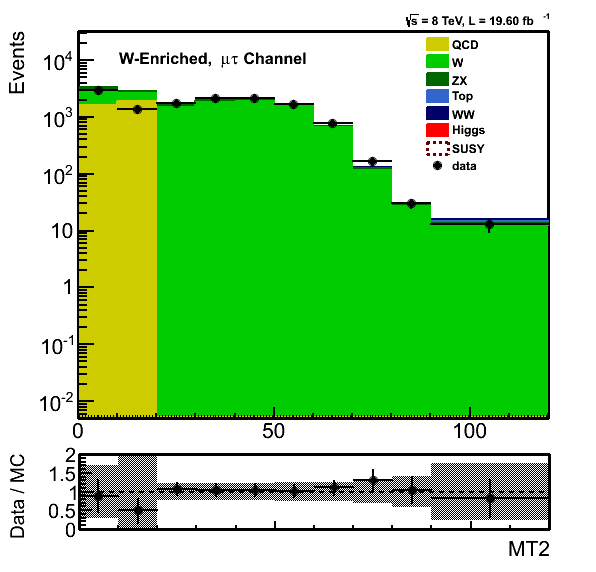
\includegraphics[angle=0,scale=0.35]{TauTauFigs/MT2_WValidation.png}
\caption{}
\label{fig:mt2_WValidation}
\end{figure}

